% The complexity classes of Chapter 8 (generated by figs_c3ch08.py).
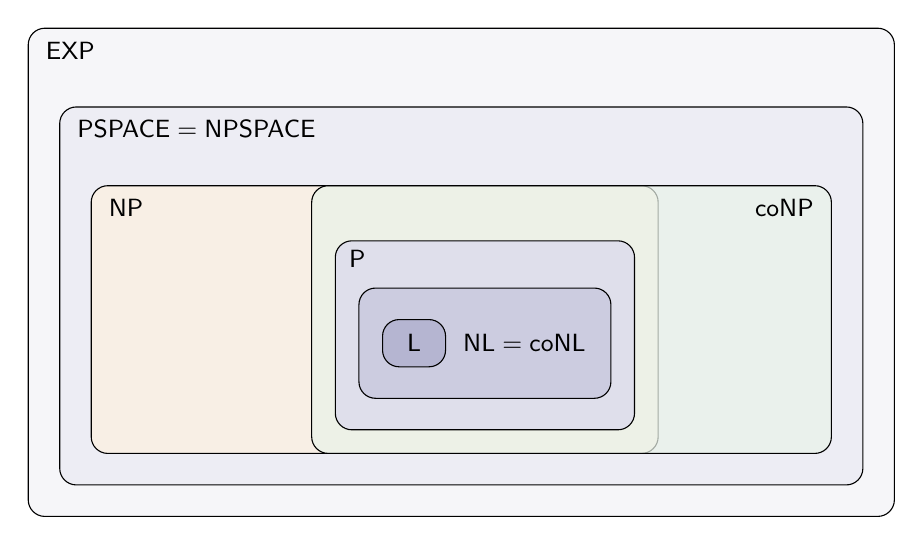
\begin{tikzpicture}[x=10mm,y=10mm,every node/.style={font=\small}]
\draw[rounded corners=6pt,fill=MidnightBlue!4] (0.0,0.0) rectangle (11.0,6.2);
\draw[rounded corners=6pt,fill=MidnightBlue!8] (0.4,0.4) rectangle (10.6,5.2);
\draw[rounded corners=6pt,fill=BurntOrange!10,fill opacity=0.7,text opacity=1] (0.8,0.8) rectangle (8.0,4.2);
\draw[rounded corners=6pt,fill=ForestGreen!10,fill opacity=0.7,text opacity=1] (3.6,0.8) rectangle (10.2,4.2);
\draw[rounded corners=6pt,fill=MidnightBlue!14] (3.9,1.1) rectangle (7.7,3.5);
\draw[rounded corners=6pt,fill=MidnightBlue!22] (4.2,1.5) rectangle (7.4,2.9);
\draw[rounded corners=6pt,fill=MidnightBlue!32] (4.5,1.9) rectangle (5.3,2.5);
\node[anchor=north west] at (0.1,6.15) {$\mathsf{EXP}$};
\node[anchor=north west] at (0.5,5.15) {$\mathsf{PSPACE}=\mathsf{NPSPACE}$};
\node[anchor=north west] at (0.9,4.15) {$\mathsf{NP}$};
\node[anchor=north east] at (10.1,4.15) {$\mathsf{coNP}$};
\node[anchor=north west] at (3.95,3.5) {$\mathsf P$};
\node[anchor=west] at (5.4,2.2) {$\mathsf{NL}=\mathsf{coNL}$};
\node at (4.9,2.2) {$\mathsf L$};
\end{tikzpicture}
